\documentclass{article}
% Change "article" to "report" to get rid of page number on title page
\usepackage{amsmath,amsfonts,amsthm,amssymb}
\usepackage{setspace}
\usepackage{Tabbing}
\usepackage{fancyhdr}
\usepackage{lastpage}
\usepackage{extramarks}
\usepackage{chngpage}
\usepackage{soul,color}
\usepackage{graphicx,float,wrapfig}
\usepackage{multirow,alltt}
\usepackage{enumerate}
% In case you need to adjust margins:
\topmargin=-0.45in      %
\evensidemargin=0in     %
\oddsidemargin=0in      %
\textwidth=6.5in        %
\textheight=9.0in       %
\headsep=0.25in         %

% Homework Specific Information
\newcommand{\hmwkTitle}{Week 7 report}
\newcommand{\hmwkClass}{}
\newcommand{\hmwkAuthorName}{Donglai\ Wei}


% Setup the header and footer
\pagestyle{fancy}                                                       %
\lhead{\hmwkAuthorName}                                                 %
\rhead{\firstxmark}                                                     %
\lfoot{\lastxmark}                                                      %
\cfoot{}                                                                %
\rfoot{Page\ \thepage\ of\ \pageref{LastPage}}                          %
\renewcommand\headrulewidth{0.4pt}                                      %
\renewcommand\footrulewidth{0.4pt}                                      %

% This is used to trace down (pin point) problems
% in latexing a document:
%\tracingall

%%%%%%%%%%%%%%%%%%%%%%%%%%%%%%%%%%%%%%%%%%%%%%%%%%%%%%%%\begin{enumerate}

% Some tools
\newcommand{\enterProblemHeader}[1]{\nobreak\extramarks{#1}{#1 continued on next page\ldots}\nobreak%
                                    \nobreak\extramarks{#1 (continued)}{#1 continued on next page\ldots}\nobreak}%
\newcommand{\exitProblemHeader}[1]{\nobreak\extramarks{#1 (continued)}{#1 continued on next page\ldots}\nobreak%
                                   \nobreak\extramarks{#1}{}\nobreak}%

\newlength{\labelLength}
\newcommand{\labelAnswer}[2]
  {\settowidth{\labelLength}{#1}%
   \addtolength{\labelLength}{0.25in}%
   \changetext{}{-\labelLength}{}{}{}%
   \noindent\fbox{\begin{minipage}[c]{\columnwidth}#2\end{minipage}}%
   \marginpar{\fbox{#1}}%

   % We put the blank space above in order to make sure this
   % \marginpar gets correctly placed.
   \changetext{}{+\labelLength}{}{}{}}%

\setcounter{secnumdepth}{0}
\newcommand{\homeworkProblemName}{}%
\newcounter{homeworkProblemCounter}%
\newenvironment{homeworkProblem}[1][Problem \arabic{homeworkProblemCounter}]%
  {\stepcounter{homeworkProblemCounter}%
   \renewcommand{\homeworkProblemName}{#1}%
   \section{\homeworkProblemName}%
   \enterProblemHeader{\homeworkProblemName}}%
  {\exitProblemHeader{\homeworkProblemName}}%

\newcommand{\problemAnswer}[1]
  {\noindent\fbox{\begin{minipage}[c]{\columnwidth}#1\end{minipage}}}%

\newcommand{\problemLAnswer}[1]
  {\labelAnswer{\homeworkProblemName}{#1}}

\newcommand{\homeworkSectionName}{}%
\newlength{\homeworkSectionLabelLength}{}%
\newenvironment{homeworkSection}[1]%
  {% We put this space here to make sure we're not connected to the above.
   % Otherwise the changetext can do funny things to the other margin

   \renewcommand{\homeworkSectionName}{#1}%
   \settowidth{\homeworkSectionLabelLength}{\homeworkSectionName}%
   \addtolength{\homeworkSectionLabelLength}{0.25in}%
   \changetext{}{-\homeworkSectionLabelLength}{}{}{}%
   \subsection{\homeworkSectionName}%
   \enterProblemHeader{\homeworkProblemName\ [\homeworkSectionName]}}%
  {\enterProblemHeader{\homeworkProblemName}%

   % We put the blank space above in order to make sure this margin
   % change doesn't happen too soon (otherwise \sectionAnswer's can
   % get ugly about their \marginpar placement.
   \changetext{}{+\homeworkSectionLabelLength}{}{}{}}%

\newcommand{\sectionAnswer}[1]
  {% We put this space here to make sure we're disconnected from the previous
   % passage

   \noindent\fbox{\begin{minipage}[c]{\columnwidth}#1\end{minipage}}%
   \enterProblemHeader{\homeworkProblemName}\exitProblemHeader{\homeworkProblemName}%
   \marginpar{\fbox{\homeworkSectionName}}%

   % We put the blank space above in order to make sure this
   % \marginpar gets correctly placed.
   }%

%%%%%%%%%%%%%%%%%%%%%%%%%%%%%%%%%%%%%%%%%%%%%%%%%%%%%%%%%%%%%



%%%%%%%%%%%%%%%%%%%%%%%%%%%%%%%%%%%%%%%%%%%%%%%%%%%%%%%%%%%%%
% Make title
\title{\vspace{0.3in}\textmd{\textbf{\hmwkTitle}}}
\date{2010.10.19}
\author{\textbf{\hmwkAuthorName}}
%%%%%%%%%%%%%%%%%%%%%%%%%%%%%%%%%%%%%%%%%%%%%%%%%%%%%%%%%%%%%

\begin{document}
\begin{spacing}{1.1}
\maketitle

\section{1) Reorganization of ME moves}
\subsection{A) Focus on Dish Config}
Inspired by Blei's "Reading Tea Leaves: How Humans Interpret Topic Models":\\
{\bf Focus on the latent space:}\\
1) How well is a certain restaurant explained by the dishes ?$\Rightarrow$ Decompose-Restaurant Move(lower level)\\
2) How representative are the dishes? $\Rightarrow$ Dish Refinement(higher level)\\ \\
So, we are going to do higher-level moves, directly refining dish config.
\subsection{B) Change}
{\bf Previously:}\\
a) We decompose a dish with the combo: Decompose-Res(Re-initialization)+Merge-Dish+Local-Dish\\
b) Accept/Reject at the end of the combo\\
{\bf Now:}\\ 
a) Treat Re-initialization, Merge-Dish and Local-Dish equally as three moves to refine dish config\\
b) Accept/Reject at the end of each move\\
\subsection{C) Efficiency}
Basically, the optimization problem has two phases:\\
1) Annealing:from {\bf Bad} to {\bf Good}\\
2) Search Until convergence: from {\bf Good} to {\bf Convergence}
\begin{enumerate}[(I)]
 \item For annealing: we may want to keep the previous order, still doing the combo but Accept/Reject by themselves
 \item For Search until convergence:\\ 
\begin{enumerate}[(1)]
 \item In Decompose-Restaurant, we may only want to re-initialize the table with the certain dish.
Otherwise, it may be too wasteful to throw away previous config which may be almost good.
 \item In Decompose-Dish, we may want to decompose noiser dishes more frequently.
 \item In Merge-Dish, we may want to merge smaller dishes more frequently.
\end{enumerate}
\end{enumerate}
\subsection{C) Pseudocode}
\begin{alltt}
  \(\%a)Annealing:\)
      For iter=1:n
          Temperature=\((\frac{iter}{n})^p\)
          For dish in {dishes} (random order):
                    Decompose-Restaurant(restaurants serving dish)
                    Local-Word(randsample(dish))
                    Merge-Dish(randsample(dish,weight))
          End
      End

  \(\%b)Run for Convergence:\)
      While Likelihood doesn't increase any more:          
          Switch(randsample([1,2,3],weight_move))
              case 1:
              \(\%1)Local Word Refinement () :\)
                    Local-Word(randsample(dish))
              case 2:
              \(\%1)Merge Dish Refinement () :\)
                    weight~num of words in the dish
                    Merge-Dish(randsample(dish,weight))
              case 3:
              \(\%1)Decompose Dish Refinement () :\)
                    weight~-Likelihood/num of words in the dish
		    Decompose-Dish(randsample(dish,weight))
	  End
      End
\end{alltt}
\subsection{D) Tests}
1) 200 restaurants, each of which is a 5 by 5 matrix(25 words) with 50 customers:\\
Initialization:\\
a) each restaurant forms its own dish\\
b) Simulation of the HDP-CRF: given $\alpha,\gamma$, we can first sample $t_{ji}$ for each restaurant and sample $k_{jt}$ for each table \\ \\
ME-anneal+ME-search-until-convergence gives perfect result \\
\emph{(Though I have to pick the annealing scheme after several tests manually.)}\\ \\
2) 200 restaurants, each of which is a 10 by 10 matrix(100 words) with 200 customers:\\
Initialization:\\
a) Gibbs Block Sampler\\ \\
ME-search-until-convergence gives perfect result
\section{2) Gibbs Sampling with FAIR INITIALIZATION}
Previously, I was scared away by the use of matlab class in Teh's code.\\ \\
I worked out the test for npbayes-r1(1st version) while npbayes-r21(2nd version) is still a little too tricky for me figure out.\\ \\
{\bf Fair Initialization:}
\begin{enumerate}[(a)]
 \item Simulation of the HDP-CRF: given $\alpha,\gamma$, we can first sample $t_{ji}$ for each restaurant and sample $k_{jt}$ for each table 
 \item Naively, each restaurant forms its own dish.
\end{enumerate}
1) I did the same test mentioned in D.1)for Gibbs Block Sampler(Teh's best sampler).\\
\emph{(Namely, 200 restaurants, each of which is a 5 by 5 matrix(25 words) with 200 customers.)}\\
Generally, the results become much noiser than their own LDA-initialization.
\begin{figure}
 \centering
   \begin{tabular}{cc}    
     \resizebox{40mm}{!}{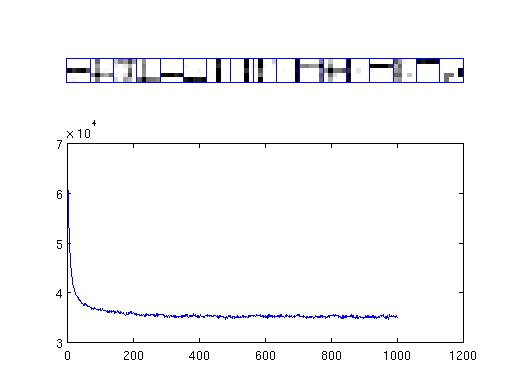
\includegraphics{hdo_block.jpg}} &
     \resizebox{40mm}{!}{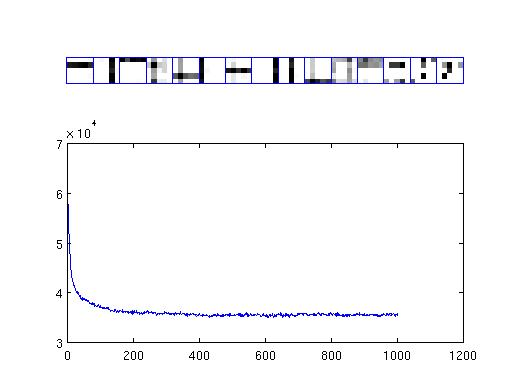
\includegraphics{all_1_block.jpg}}\\ 
        \end{tabular}
    \caption{5 by 5 matrix left: initialization a); right: initialization b)}
    \label{fig:by:table} 
\end{figure}
2) I run it for a larger data set: 1000 restaurants, each of which is a 30 by 30 matrix(900 words) with 1800 customers.)\\
It only finds 30+ dishes, many of which are either noisy or composition of bars.
\begin{figure}
 \centering
     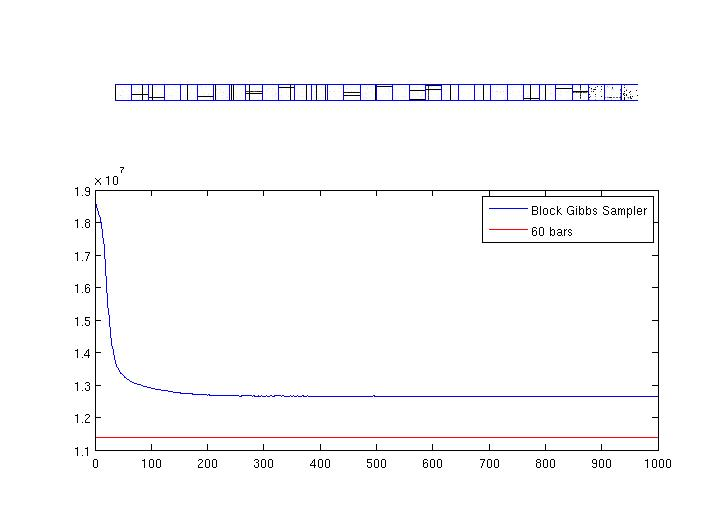
\includegraphics[width=5in,height=3in]{30_block.jpg}
    \caption{30 by 30 matrix The Gibbs Block Sampler Breaks down}
    \label{fig:by:table} 
\end{figure}

\newpage
\section{3) Results on Topic Model}
Here, I run Gibbs Sampling and ME algorithm on a synthetic data from NIPS abstract: 100 words and 200 documents, each of which has around 200 words.\\
\emph{Similar size to that of previous bar test, but it is much more harder}
\subsection{a) Gibbs Sampler totally falls}
Given the documents, intuitively, topic selection sucks if:
\begin{enumerate}
 \item The algorithm gives too many topics
 \item Each topic is a noisy combination of different words
\end{enumerate}
Gibbs CRF sampler (though we know already it's no good) gives 178 topics.\\
Though Gibbs Block sampler gives only 32 topics, the average number of different types of words for each topic is 41.\\ \\
\begin{figure}
 \centering
     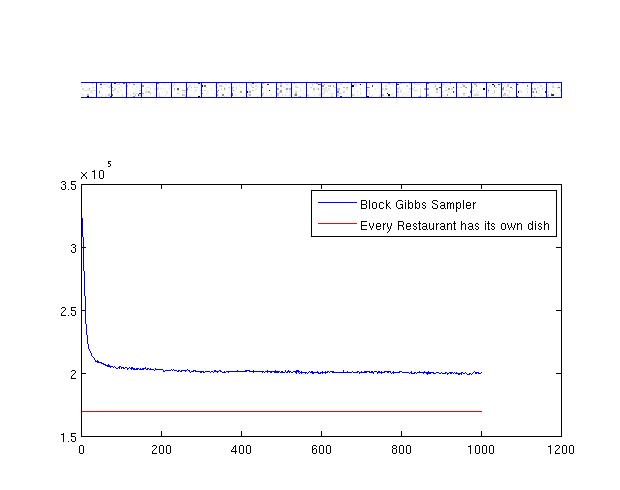
\includegraphics[width=5in,height=3in]{topic_block.jpg}
    \caption{Gibbs Block Sampler on the synthetic topic data}
    \label{fig:by:table} 
\end{figure}
\newpage
\subsection{b) ME annealing}
1) If we directly run ME after Gibbs Block Sampler, the likelihood will go up by making each restaurant a table, which is typical
bad situation when the dish config is unclear and the gain only comes from maximizing t-term.\\ \\
2) So we have to run annealing version of ME algorithm. When T is small, Decompose-Restaurant tends to have more restaurants. 
With the increase of the Temperature, t-term and k-term gradually come to the balance. \\ \\
It's still running....taking so long...
\end{spacing}
\end{document}

%%%%%%%%%%%%%%%%%%%%%%%%%%%%%%%%%%%%%%%%%%%%%%%%%%%%%%%%%%%%%
